\documentclass[12pt, a4paper]{article}

% Кодировка и язык
\usepackage[utf8]{inputenc}
\usepackage[russian]{babel}

% Математика и шрифты
\usepackage{amsmath, amssymb}
\usepackage{mathtools}
\usepackage{pdflscape}

% Графика и расположение картинок
\usepackage{graphicx}
\usepackage{float} % Для точного позиционирования [H]
\usepackage{subcaption} % Для подписей к подрисункам (если понадобится)

% Геометрия страницы
\usepackage[left=2cm, right=2cm, top=2cm, bottom=2cm]{geometry}

% Гиперссылки
\usepackage{hyperref}
\hypersetup{
	colorlinks=true,
	linkcolor=blue,
	filecolor=magenta,      
	urlcolor=cyan,
}
%======================================================================================
\makeatletter
% Изменяем направление поворота контента
\patchcmd{\LS@rot}{90}{-90}{}{}
% Изменяем атрибут поворота страницы в PDF
\patchcmd{\landscape}{\PLS@Rotate{90}}{\PLS@Rotate{-90}}{}{}
\makeatother

\begin{document}
	

	\section{Введение и формализация модели}
	
	В данной работе исследуется процесс роста кристаллических структур с использованием двумерных клеточных автоматов (КА). Клеточные автоматы представляют собой дискретные модели, эволюционирующие во времени по локальным правилам, и являются мощным инструментом для изучения эмерджентности --- возникновения сложных глобальных структур из простых взаимодействий.
	
	Формально классический клеточный автомат задается как кортеж $\langle A, S, N, F \rangle$ (согласно п. 2 лекции):
	\begin{itemize}
		\item \textbf{$A$ (Пространство):} Двумерная квадратная решетка размером $M \times N$. В экспериментах использовались поля $300 \times 300$ и $400 \times 400$.
		\item \textbf{$S$ (Состояния):} Дискретный набор состояний клетки $s_{ij} \in \{0, 1, 2\}$, где $0$~--- пустота (раствор), $1$~--- частица кристалла, $2$~--- неподвижное препятствие.
		\item \textbf{$N$ (Окрестность):} В работе исследованы два типа окрестностей (п. 2.1):
		\begin{itemize}
			\item \textit{Фон Неймана} (4 ортогональных соседа).
			\item \textit{Мура} (8 соседей, включая диагонали).
		\end{itemize}
		\item \textbf{$F$ (Правило перехода):} Локальное однородное правило, зависящее от выбранной физической модели (DLA или Eden).
		\item \textbf{Граничные условия (п. 2.2):} Фиксированные (частицы, ушедшие за пределы решетки, удаляются из симуляции).
	\end{itemize}
	
	\section{Исследуемые алгоритмы роста}
	
	Для сравнения механизмов кристаллизации были реализованы две фундаментально разные модели.
	
	\subsection{Модель DLA (Diffusion-Limited Aggregation)}
	Моделирует рост, ограниченный диффузией (например, электроосаждение или рост снежинок). 
	\begin{itemize}
		\item \textbf{Алгоритм:} Частица запускается на периферии кластера и совершает случайное блуждание (random walk). Если в её окрестности $N$ оказывается занятая клетка ($s=1$ или $s=2$), частица необратимо прилипает ($s \leftarrow 1$).
		\item \textbf{Ожидаемая морфология:} Фрактальные, дендритные структуры с размерностью $D \approx 1.7$.
	\end{itemize}
	
	\subsection{Модель Эдема (Eden Model)}
	Моделирует аккреционный рост (например, рост бактериальной колонии), где новые элементы добавляются только на границу кластера.
	\begin{itemize}
		\item \textbf{Алгоритм:} Поддерживается список свободных клеток, граничащих с кристаллом (boundary). На каждом шаге случайно выбирается одна такая клетка и становится частью кристалла. Список границы обновляется.
		\item \textbf{Ожидаемая морфология:} Плотный, компактный кластер с размерностью $D \to 2.0$.
	\end{itemize}
	
	\section{Эксперимент 1: Сравнение механизмов роста (DLA vs Eden)}
	
	На рисунке \ref{fig:comparison} представлено сравнение морфологии кластеров, полученных двумя разными методами, а также график зависимости радиуса кластера от числа частиц в логарифмических координатах.
\begin{landscape}
	\begin{figure}[H]
		\centering
		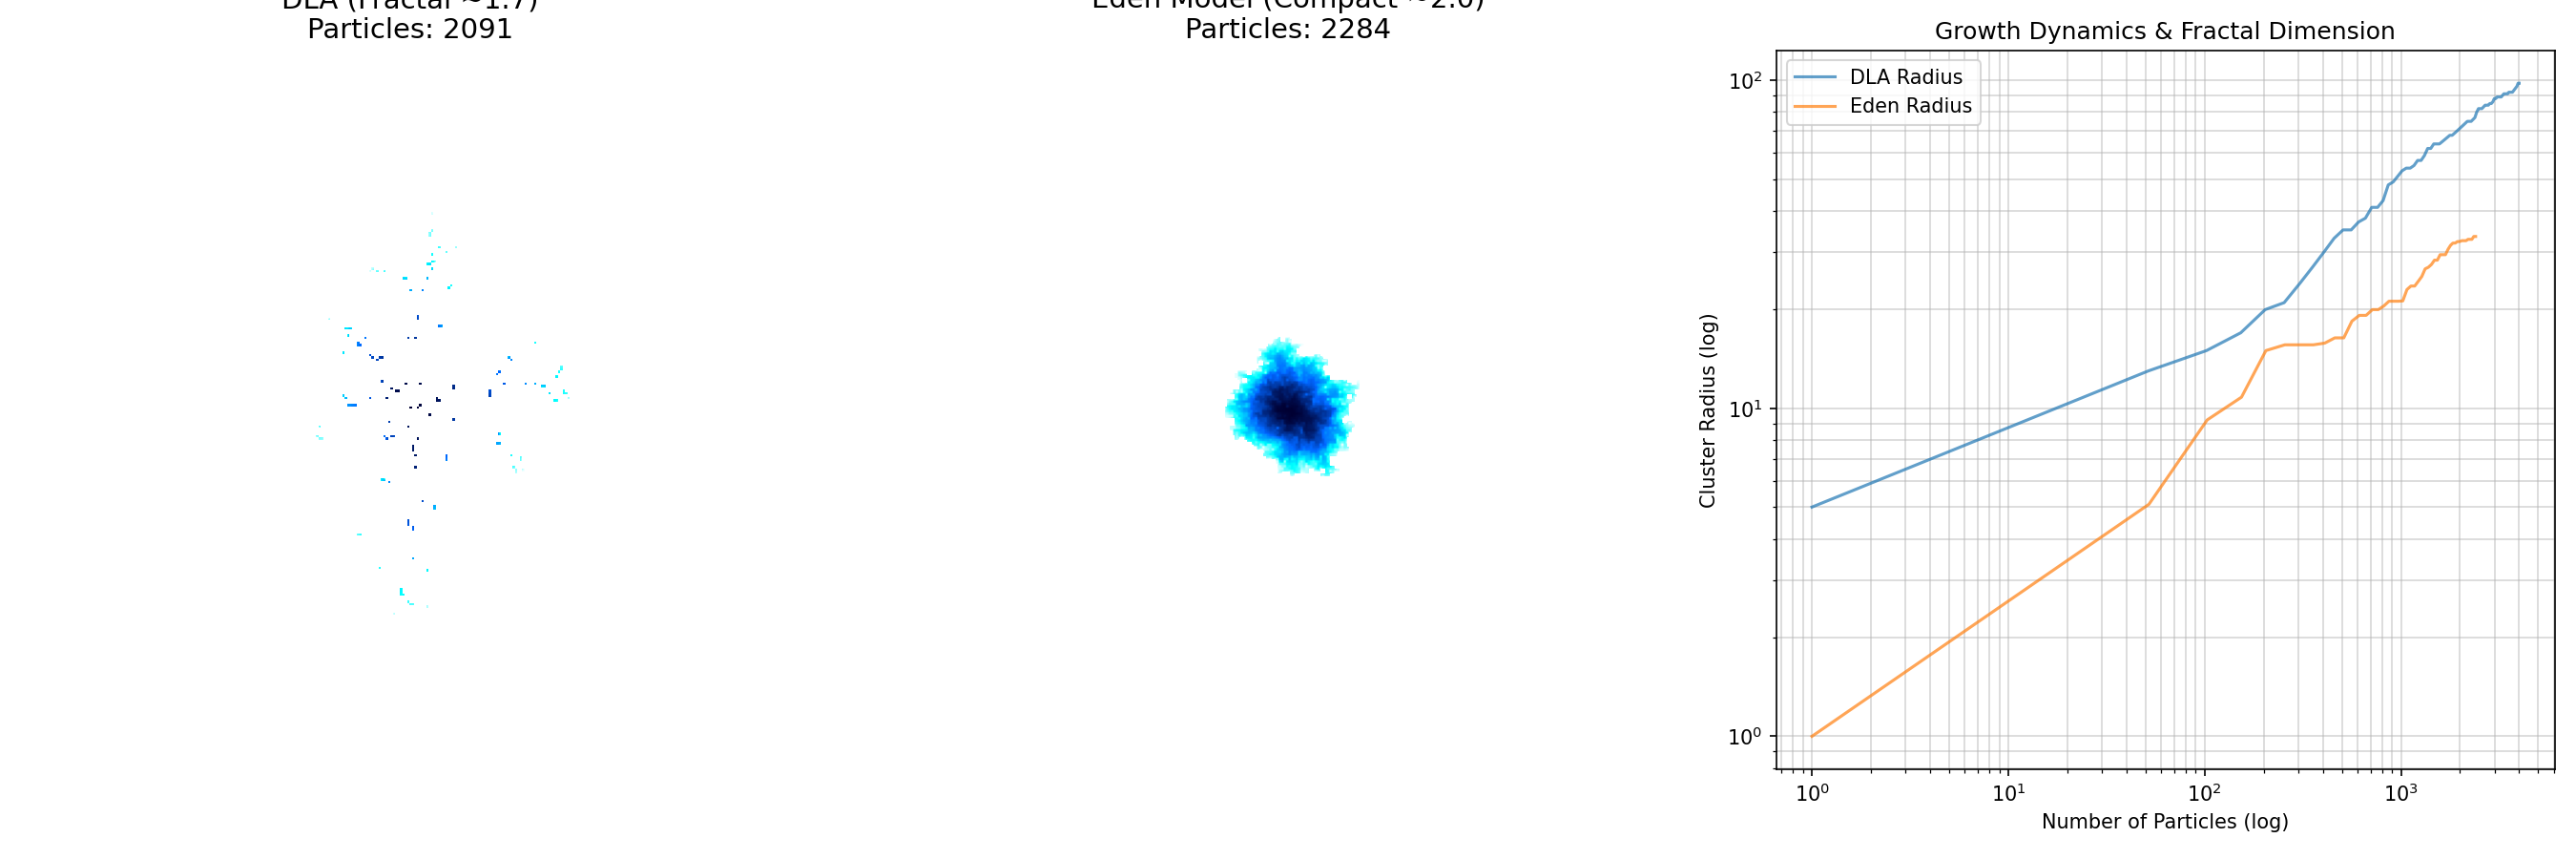
\includegraphics[width=1.5\textwidth]{comparison_final.png}
		\caption{Сравнение моделей роста. Слева: DLA (фрактальная структура). В центре: Модель Эдема (компактный рост). Справа: Динамика роста радиуса (Log-Log scale). Наклон линий отражает фрактальную размерность.}
		\label{fig:comparison}
	\end{figure}
\end{landscape}	
	
	\textbf{Анализ результатов:}
	\begin{itemize}
		\item \textbf{DLA:} Образует разреженный фрактал с длинными ветвями. График зависимости (синяя линия) имеет больший наклон, что соответствует меньшей фрактальной размерности. Ветви экранируют внутреннюю область, не давая новым частицам проникать в центр (эффект экранирования).
		\item \textbf{Eden:} Образует плотный кластер. Оранжевая линия на графике имеет меньший наклон, стремясь к размерности 2. Рост происходит равномерно по всему фронту поверхности.
	\end{itemize}
	
	\textbf{Вывод:} Тип транспорта частиц (диффузия из объема vs присоединение к поверхности) фундаментально меняет макроскопическую структуру, демонстрируя эмерджентность (п. 3.6, 4.7 лекции).
	
	\section{Эксперимент 2: Влияние типа окрестности}
	
	В рамках модели Эдема было исследовано влияние топологии связей на форму кристалла (п. 2.1, 6.2 лекции).
	
\begin{landscape}
	\begin{figure}[H]
		\centering
		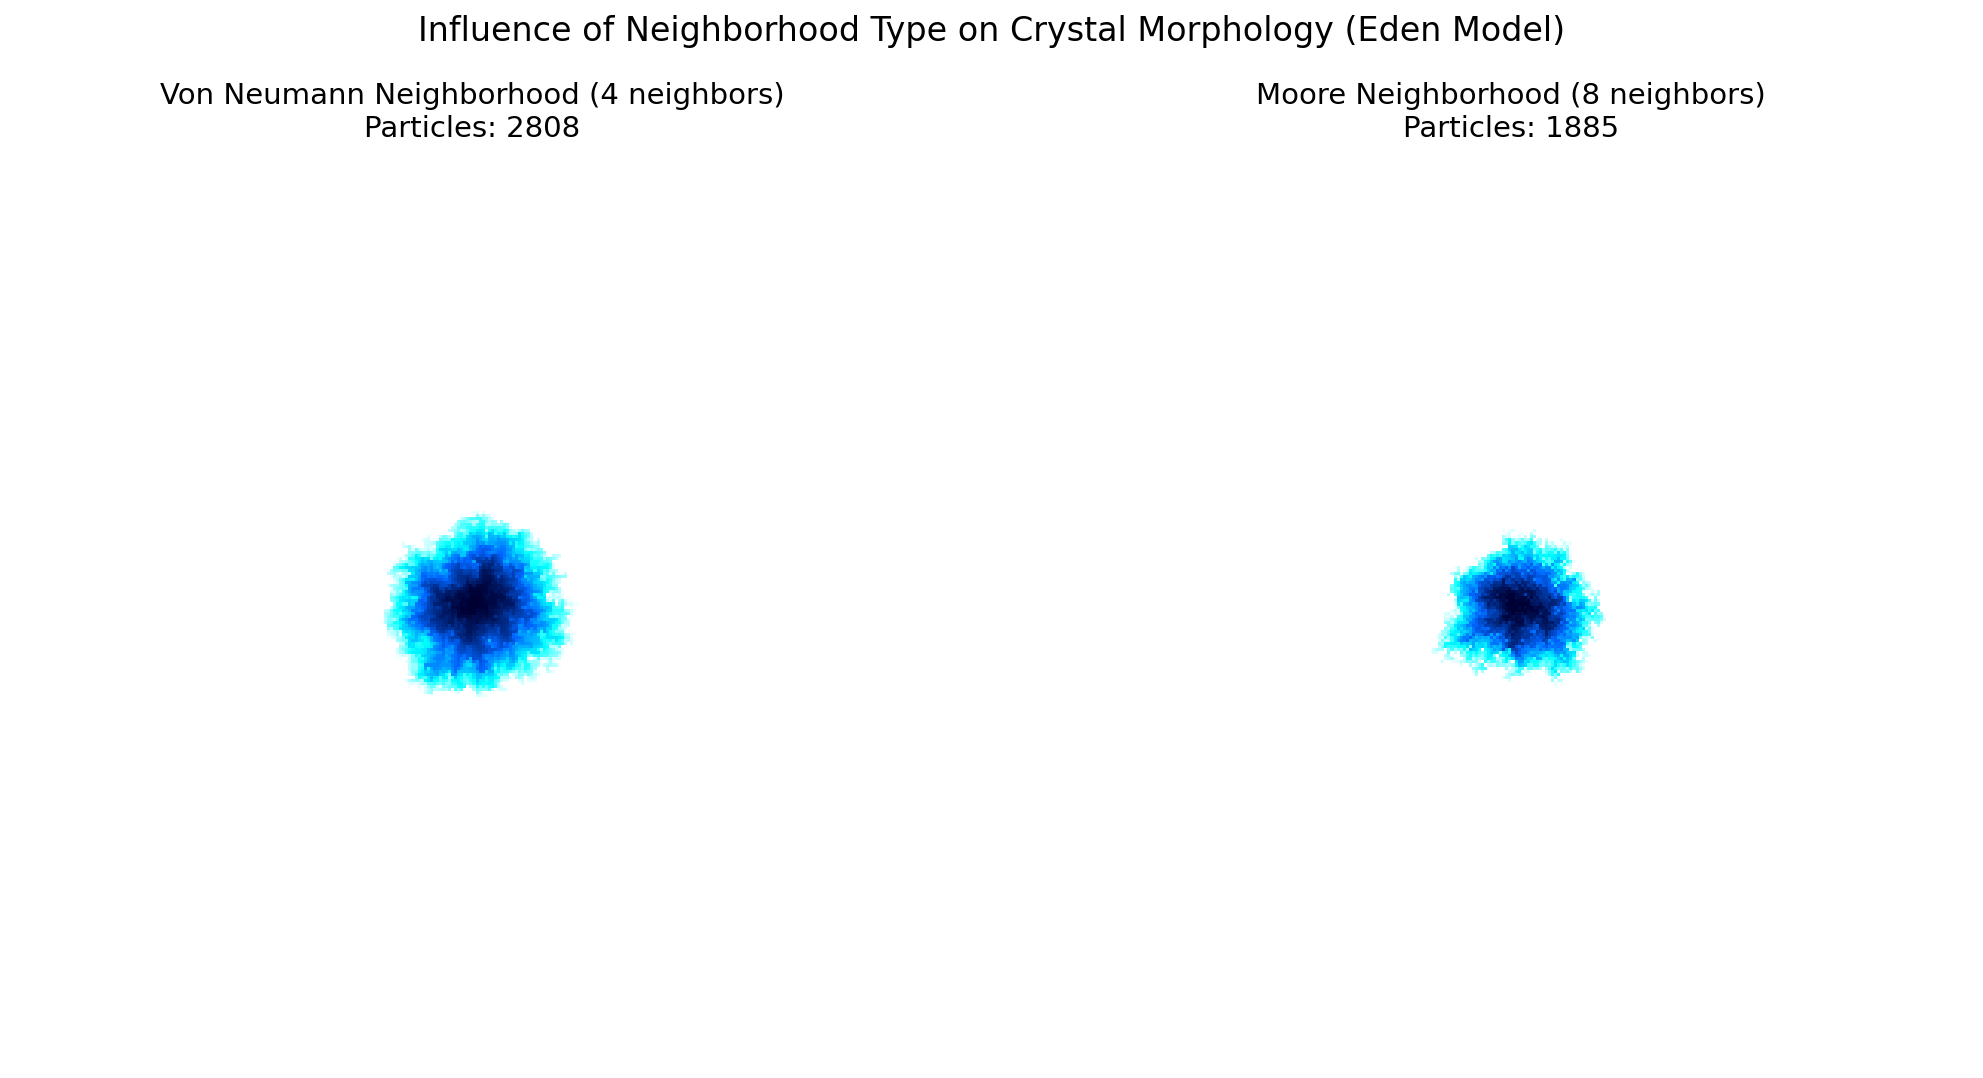
\includegraphics[width=1.5\textwidth]{neighborhood_comparison.png}
		\caption{Влияние окрестности на модель Эдема. Слева: Фон Нейман (4 соседа). Справа: Мур (8 соседей).}
		\label{fig:neighborhood}
	\end{figure}
\end{landscape}
	
	\textbf{Анализ результатов:}
	При переходе от окрестности фон Неймана к окрестности Мура глобальная компактность структуры сохраняется. Однако микроструктура границы изменяется: наличие диагональных связей (окрестность Мура) делает фронт роста чуть более изотропным (округлым) и увеличивает скорость заполнения пространства (что видно по разнице в количестве частиц за фиксированное время итераций).
	
	\textbf{Вывод:} Модель Эдема демонстрирует высокую устойчивость (п. 3.9.4) к изменению типа окрестности на макроуровне, в отличие от DLA, где тип окрестности критически влияет на толщину ветвей.
	
	\section{Эксперимент 3: Рост в неоднородной среде («Кристалл в лабиринте»)}
	
	Для исследования влияния начальных условий и пространственных ограничений (п. 6.2) в модель DLA было добавлено кольцевое препятствие с единственным узким разрывом (п. 3.9.4 --- добавление препятствия).
\begin{landscape}
	\begin{figure}[H]
		\centering
		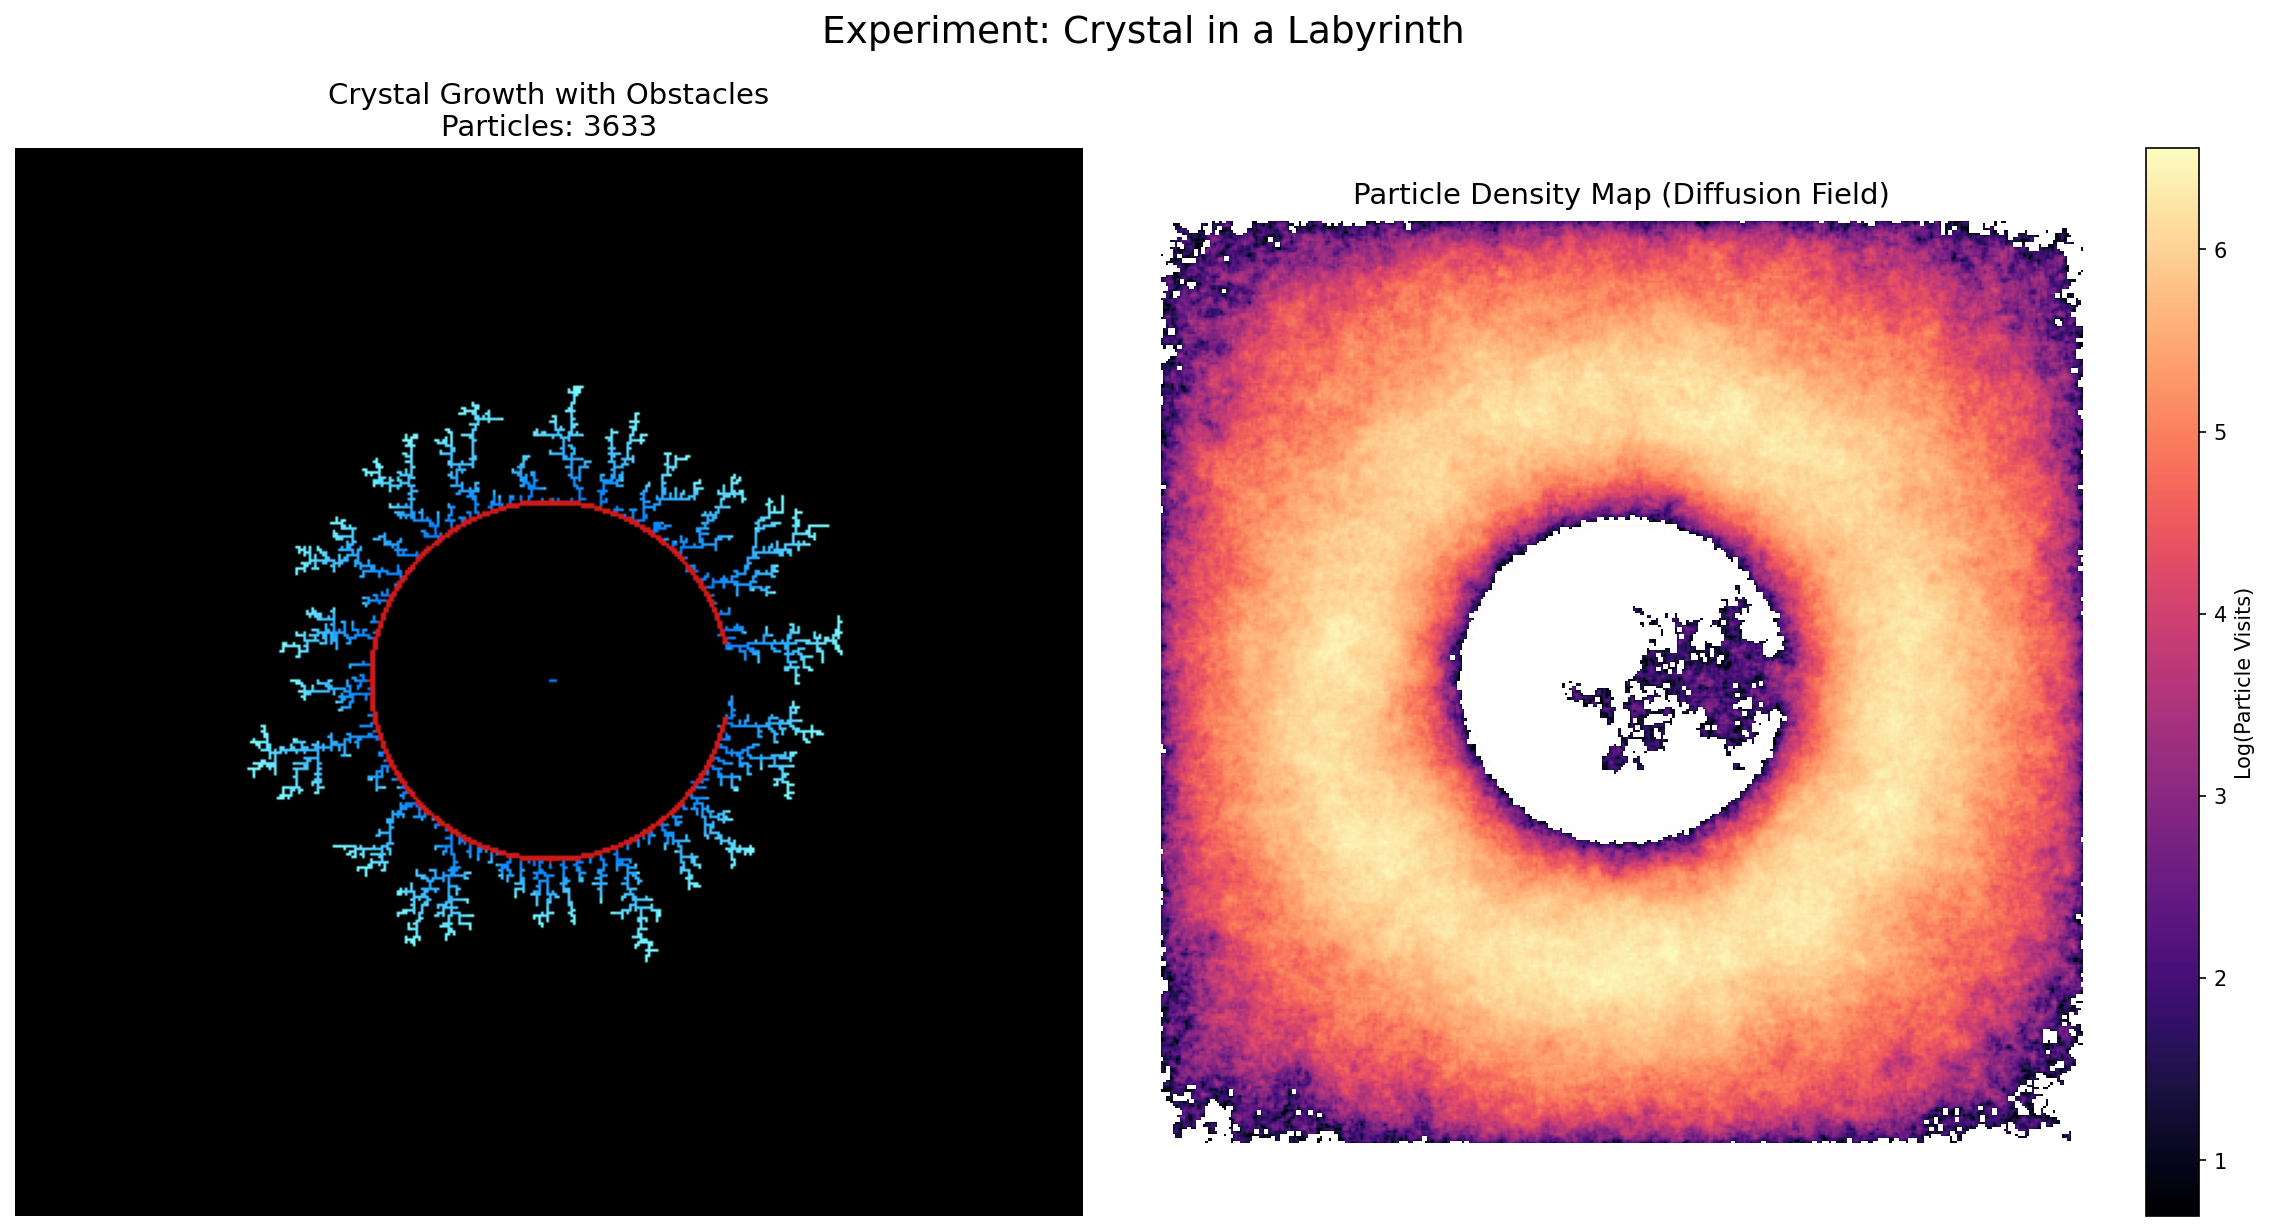
\includegraphics[width=1.5\textwidth]{labyrinth_experiment.png}
		\caption{Рост кристалла с препятствием. Слева: Структура кластера (красный цвет --- препятствие). Справа: Тепловая карта посещений клеток (логарифмическая шкала), визуализирующая поле диффузии.}
		\label{fig:labyrinth}
	\end{figure}
\end{landscape}
	\textbf{Анализ результатов:}
	\begin{itemize}
		\item \textbf{Структурный анализ:} Кристалл успешно формирует сложную структуру, «обтекая» внешнюю сторону препятствия. Через узкую щель наблюдается прорастание единичных ветвей во внутреннюю полость, где формируется вторичный, значительно меньший кластер.
		\item \textbf{Анализ поля диффузии:} Построена тепловая карта посещений клеток блуждающими частицами (рис. \ref{fig:labyrinth}, справа). Ярко выражена зона высокой плотности (оранжевый ореол) вокруг внешней стенки препятствия. Внутренняя область кольца находится в «диффузионной тени» (низкая плотность посещений), что физически объясняет медленный рост внутреннего кластера.
	\end{itemize}
	
	\textbf{Вывод:} Пространственные ограничения радикально меняют динамику роста. Возникает эффект экранирования, который невозможно предсказать аналитически без проведения имитационного моделирования (п. 5 лекции).
	
	\section{Заключение}
	
	В ходе выполнения домашнего задания были разработаны и программно реализованы алгоритмы клеточных автоматов для моделирования роста кристаллов.
	\begin{enumerate}
		\item Проведено сравнение диффузионного (DLA) и аккреционного (Eden) механизмов, показана зависимость фрактальной размерности от правил перехода.
		\item Исследовано влияние окрестности (фон Нейман / Мур) на морфологию кластера.
		\item Проведен оригинальный эксперимент с ростом в пространстве с препятствиями, визуализировано диффузионное поле и эффект экранирования.
	\end{enumerate}
	
	Работа наглядно подтверждает тезис лекции о том, что простые локальные правила взаимодействия элементов приводят к возникновению сложных, непредсказуемых глобальных структур (эмерджентности). Как отмечено в методологических замечаниях (п. 5), «единственный способ выяснить, как эволюционирует система, заключается в наблюдении (моделировании) всех шагов её изменения», что и было успешно продемонстрировано в ходе работы.
	

	
\end{document}